\documentclass{article}
\textheight 23.5cm \textwidth 15.8cm
%\leftskip -1cm
\topmargin -1.5cm \oddsidemargin 0.3cm \evensidemargin -0.3cm
%\documentclass[final]{siamltex}

\usepackage{ctex}
\usepackage{verbatim}
\usepackage{fancyhdr}
\usepackage{graphicx}
\usepackage{amsmath}
\usepackage{amssymb}
\usepackage{float}
\usepackage{multirow}
\usepackage{colortbl}
\usepackage{amsthm}
\usepackage{bm}
\usepackage{tikz}

\textheight 23.5cm \textwidth 15.8cm
\topmargin -1.5cm \oddsidemargin 0.3cm \evensidemargin -0.3cm
\title{HW2 实验报告}
\author{PB20010429 侯相龙}

\begin{document}
\maketitle
\section{实验内容}
实现图像变形 Image warping

\section{实验原理}
基于Radial basis functions对图像的坐标点做如下变换
\begin{equation}
    f(\boldsymbol{x}) =\boldsymbol{x}+\sum_{i=1}^{n} a_{i} b_{i}(\boldsymbol{x})
\end{equation}
    
其中,
\[
    b_{i}(\boldsymbol{x}) =\frac{1}{\left|\boldsymbol{x}-\boldsymbol{p}_{i}\right|^{2}+d}
\]
d为常数,  $\boldsymbol{p}_{i}$  为约束点,  $\boldsymbol{a}_{i}$为变量通过求解以下方程组获得:

\[f\left(\boldsymbol{p}_{i}\right)=\boldsymbol{q}_{i}, i=1 \ldots n\]

\section{算法介绍与步骤}

\subsection{计算系数矩阵}
通过约束条件,计算系数矩阵A

\subsection{实现点的变幻}
在求得系数矩阵后,可以用(1)式求得任意点变换后的坐标。

\subsection{去除黑点的方法}
注意到,黑点的产生是由于两张图像间的映射并不是满射。
从而目标图像的会出现黑点(默认值0)的情况。

有下面两种方法

(1)保持原映射不变,用黑点(默认为0)周围的有颜色的点做插值填充黑点

(2)考虑原映射的“逆映射”,这样能保证新图像中的每一个点都可以被赋值。
(若非单射则考虑循环中最近一次的填充作为逆)



\section{测试数据与实验结果}
\subsection{未进行去黑点处理}



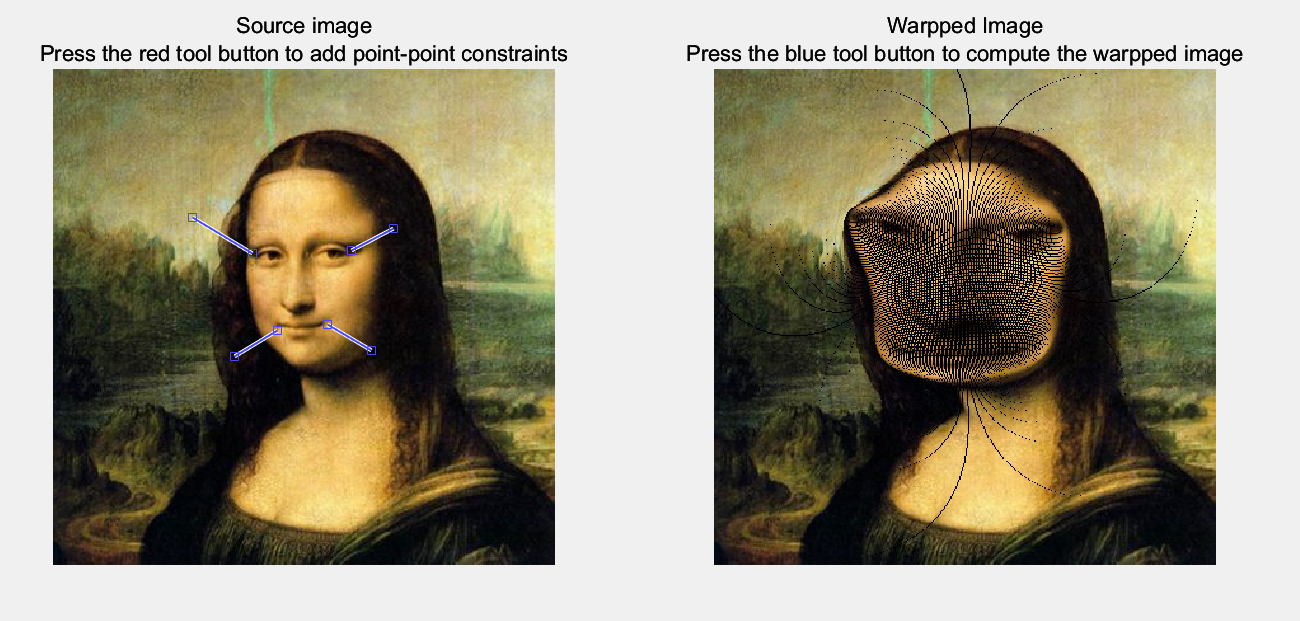
\includegraphics[width=0.6\textwidth]{1}


\subsection{去除了黑点}

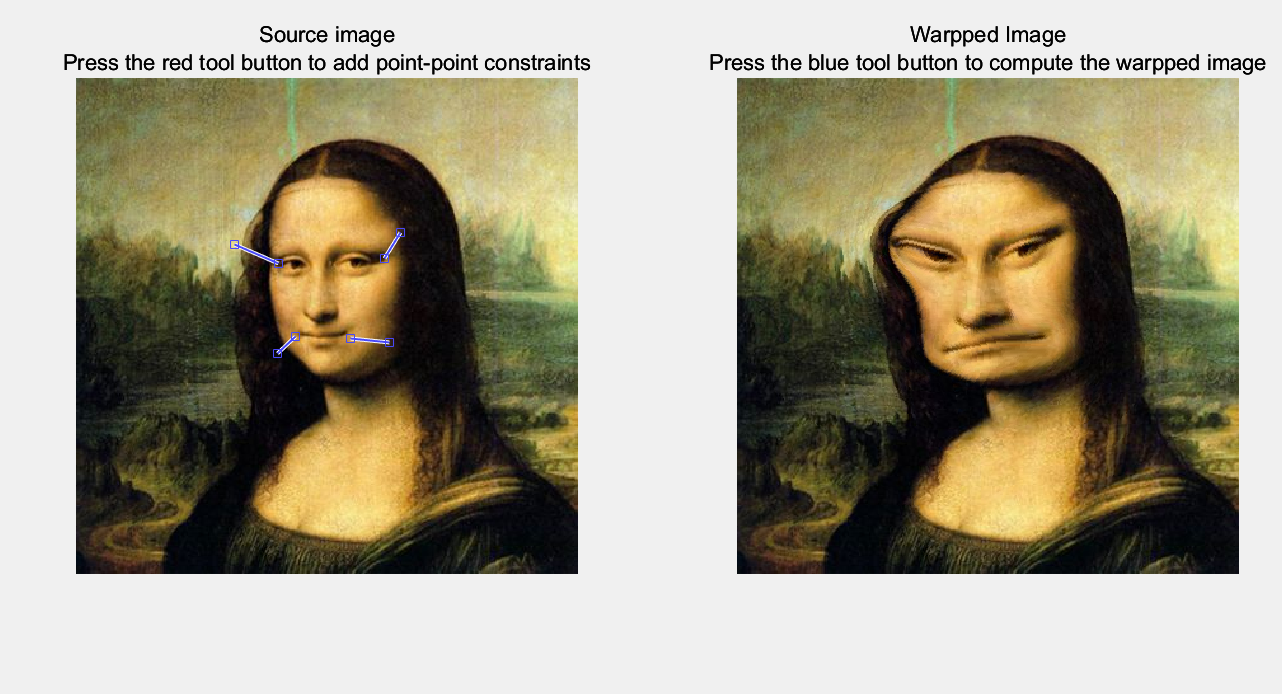
\includegraphics[width=0.6\textwidth]{3}

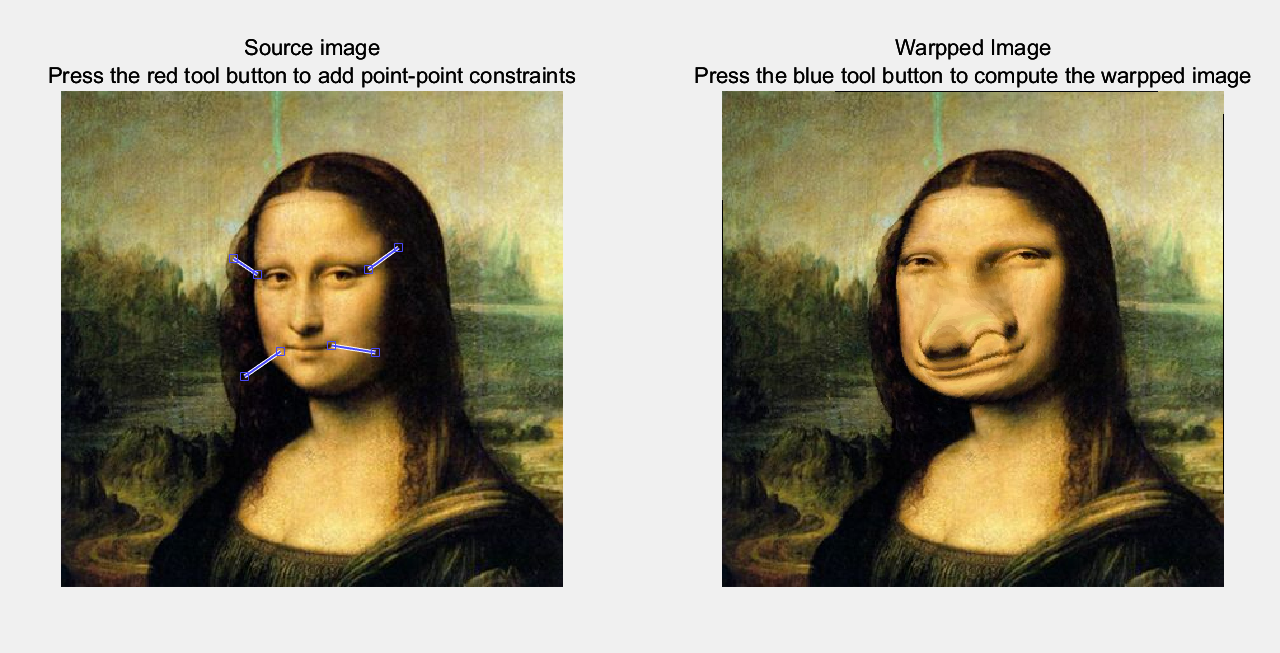
\includegraphics[width=0.6\textwidth]{2}


\end{document}
